\subsection{Geometric description of the cross product}

The following is the geometric description of the cross
product. Recall that the dot product of two vectors results in a
scalar. In contrast, the cross product results in a vector, as the
cross product gives a direction as well as a magnitude.%
\index{cross product!geometric description}

\begin{definition}{Geometric definition of cross product}{cross-product-geometric}
  Let\/ $\vect{u}$ and $\vect{v}$ be two vectors in $\R^3$. Their
  \textbf{cross product}%
  \index{cross product}, written $\vect{u}\times \vect{v}$, is the
  vector defined by the following three rules.%
  \index{cross product!geometric description}

  \begin{enumerate}
  \item Its length is $\norm{\vect{u}\times \vect{v}} =\norm{\vect{u}} \norm{
      \vect{v}} \sin \theta$,
    where $\theta $ is the included angle between $\vect{u}$ and $\vect{v}$.

  \item It is orthogonal to both $\vect{u}$ and $\vect{v}$.

  \item The vectors $\vect{u}$, $\vect{v}$, and $\vect{u}\times
    \vect{v}$, in that order, form a right-handed system.
  \end{enumerate}
\end{definition}

We note that the length of the cross product,
$\norm{\vect{u}\times\vect{v}}$, given by the formula
$\norm{\vect{u}}\norm{\vect{v}}\sin\theta$, is the area of the
parallelogram determined by $\vect{u}$ and $\vect{v}$, as shown in the
following picture.%
\index{cross product!area of parallelogram}%
\index{area!of parallelogram}%
\index{parallelogram!area of}%
\begin{center}
  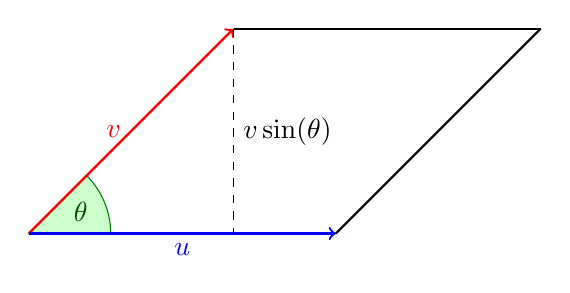
\begin{tikzpicture}[scale=1.3]
    \filldraw[fill=green!20,draw=green!50!black] (0,0) -- (0:8mm) arc (0:45:8mm) -- cycle;
    \draw[->,thick,red] (0,0) -- node[left] {$\vect{v}$} (2,2);
    \draw[->,thick,blue] (0,0) -- node[below] {$\vect{u}$} (3,0);
    \draw[thick] (2,2)--(5,2);
    \draw[thick] (3,0)--(5,2);
    \draw[dashed] (2,2)--(2,0);
    \node[green!30!black] at (22.5:5.5mm) {$\theta$};
    \node[right] at (2,1){$\norm{\vect{v}} \sin(\theta)$};
  \end{tikzpicture}
\end{center}
